%%%%%%%%%%%%%%%%%%%%%%%%%%%%%%%%%%%%%%%%%
% baposter Portrait Poster
% LaTeX Template
% Version 1.0 (15/5/13)
%
% Created by:
% Brian Amberg (baposter@brian-amberg.de)
%
% This template has been downloaded from:
% http://www.LaTeXTemplates.com
%
% License:
% CC BY-NC-SA 3.0 (http://creativecommons.org/licenses/by-nc-sa/3.0/)
%
%%%%%%%%%%%%%%%%%%%%%%%%%%%%%%%%%%%%%%%%%

%----------------------------------------------------------------------------------------
%	PACKAGES AND OTHER DOCUMENT CONFIGURATIONS
%----------------------------------------------------------------------------------------

\documentclass[a0paper,portrait]{baposter}

\usepackage[font=small,labelfont=bf]{caption} % Required for specifying captions to tables and figures
\usepackage{booktabs} % Horizontal rules in tables
\usepackage{relsize} % Used for making text smaller in some places
\usepackage[utf8]{inputenc}
\usepackage{amsmath}
\usepackage{amsfonts}
\usepackage{amssymb}
\usepackage{mathtools}
\graphicspath{{figures/}} % Directory in which figures are stored
\usepackage{booktabs}
\definecolor{bordercol}{RGB}{40,40,40} % Border color of content boxes
\definecolor{headercol1}{RGB}{186,215,230} % Background color for the header in the content boxes (left side)
\definecolor{headercol2}{RGB}{80,80,80} % Background color for the header in the content boxes (right side)
\definecolor{headerfontcol}{RGB}{0,0,0} % Text color for the header text in the content boxes
\definecolor{boxcolor}{RGB}{186,215,230} % Background color for the content in the content boxes

\begin{document}



\background{ % Set the background to an image (background.pdf)
\begin{tikzpicture}[remember picture,overlay]
\draw (current page.north west)+(-2em,2em) node[anchor=north west]
{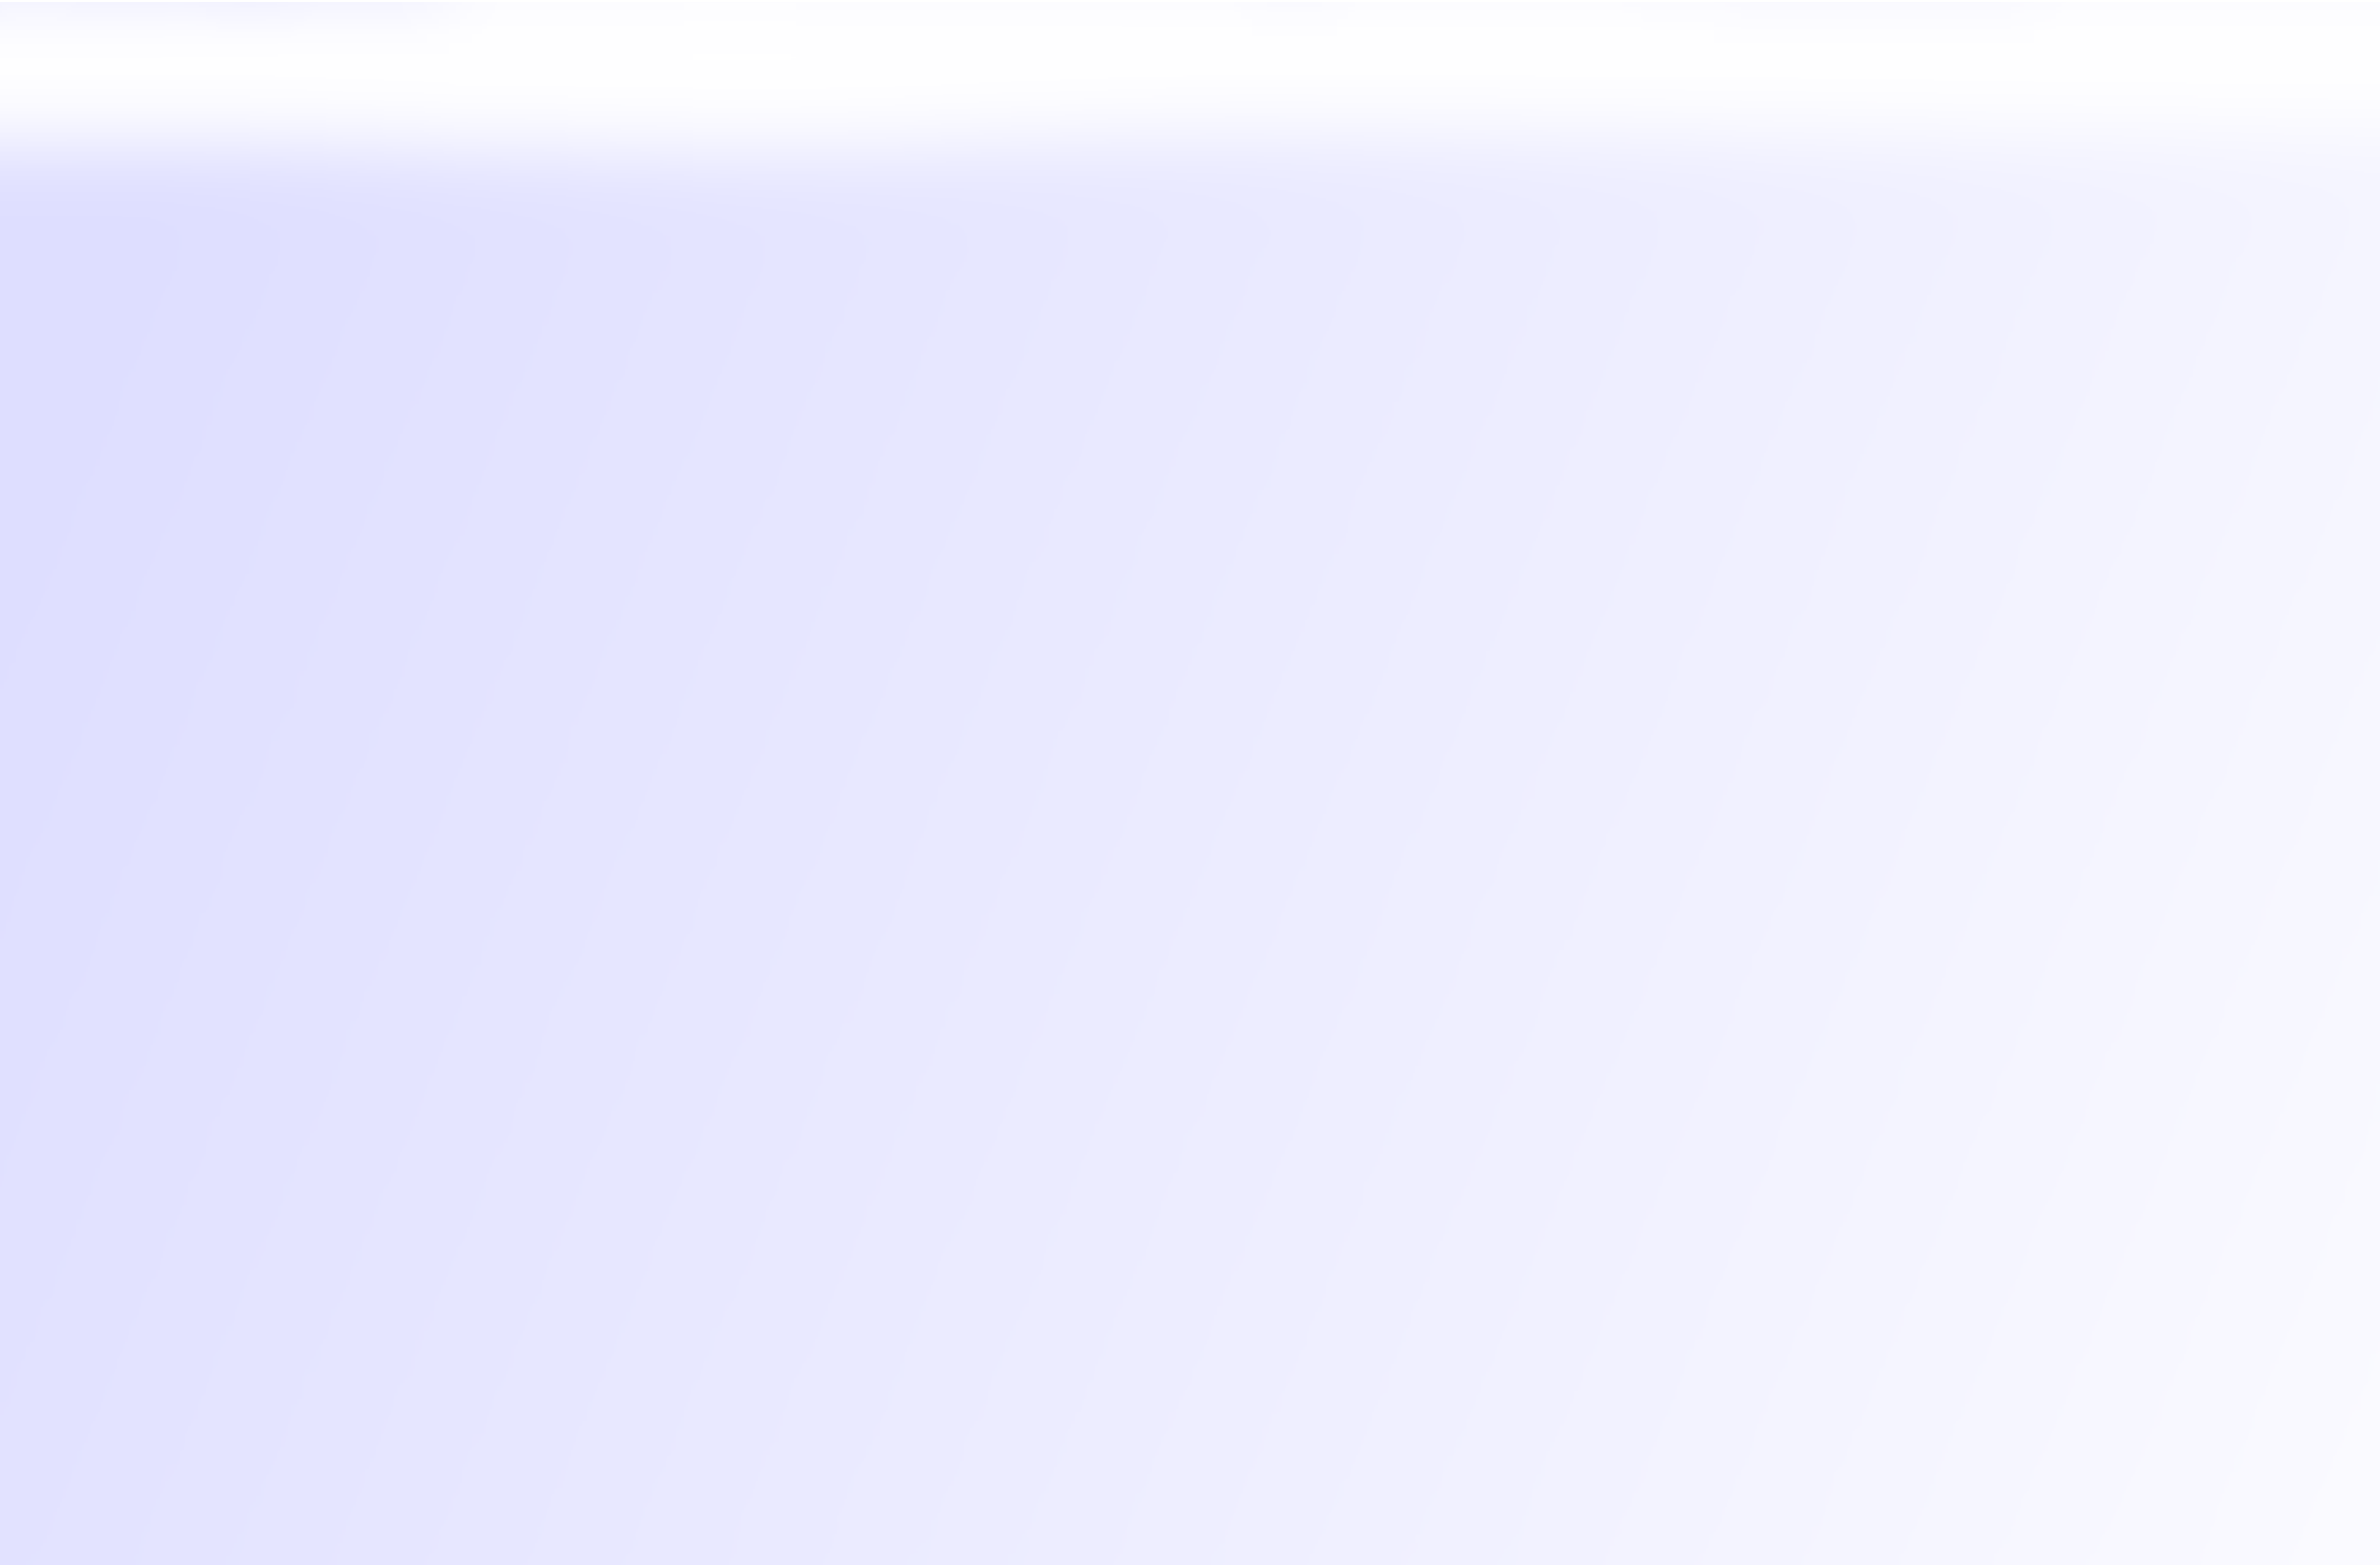
\includegraphics[height=1.1\textheight]{background}};
\end{tikzpicture}
}

\begin{poster}{
grid=false,
borderColor=bordercol, % Border color of content boxes
headerColorOne=headercol1, % Background color for the header in the content boxes (left side)
headerColorTwo=headercol2, % Background color for the header in the content boxes (right side)
headerFontColor=headerfontcol, % Text color for the header text in the content boxes
boxColorOne=boxcolor, % Background color for the content in the content boxes
headershape=roundedright, % Specify the rounded corner in the content box headers
headerfont=\Large\sf\bf, % Font modifiers for the text in the content box headers
textborder=rectangle,
background=user,
headerborder=open, % Change to closed for a line under the content box headers
boxshade=plain
}
{}
%
%----------------------------------------------------------------------------------------
%	TITLE AND AUTHOR NAME
%----------------------------------------------------------------------------------------
%
{\sf\bf \\ Sistema para la detección de faltas basado\\ en redes neuronales artificiales. Caso de aplicación: daños estructurales} % Poster title
{\vspace{0.5em} Jeferson González, Yeiner Arias\\ % Author names
{\smaller jgonzalez@itcr.ac.cr, yarias@itcr.ac.cr}} % Author email addresses
{
\includegraphics[scale=0.6]{logo}} % University/lab logo

%----------------------------------------------------------------------------------------
%	INTRODUCTION
%----------------------------------------------------------------------------------------

\headerbox{Introducción}{name=introduction,column=0,row=0}{
\begin{footnotesize}

El análisis de vibración es una técnica utilizada para el estudio de los efectos dinámicos en estructuras y la evaluación de posibles daños. Ésta se ubica dentro de la categoría de ensayos no destructivos, lo cual es un aspecto importante en estructuras de costo elevado y donde las pruebas destructivos no son una alternativa. \\

Las señales de vibración son procesadas mediante un algoritmo digital que permite extraer información relevante por media de la Transformada Discreta de Fourier (DFT) que es un mecanismo de análisis de frecuencia para señales no periódicas. \\


Una red neuronal artificial es un modelo simplificado del sistema neuronal humano. La unidad básica de una red neuronal se llama \textbf{neurona artificial}, cuya función de salida es:
\end{footnotesize}

\begin{equation}
\sum_{i=1}^{N} x_i w_{ji} + b
\end{equation}

%\begin{center}
%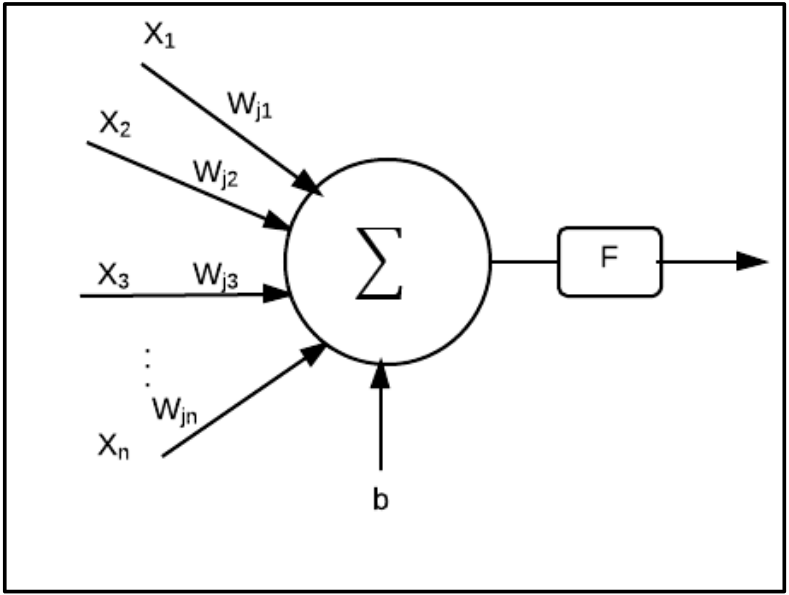
\includegraphics[width=0.49\linewidth]{neurona}
%\\ {\footnotesize \textbf{Figura 1.} Neurona artifical.}
%\end{center}

\begin{footnotesize}
Con la correcta distribución de capas de neuronas simples, un red neuronal artifical puede utlizarse para diferentes aplicaciones como lo son la identificación de señales/funciones y la \textbf{detección de patrones}. \\

La detección de faltas en sistemas, en general, requiere una distribución de capas y neuronas que les permita \textbf{aprender} el comportamiento del sistema tanto en condiciones normales como en falta. 
\end{footnotesize}
\begin{center}
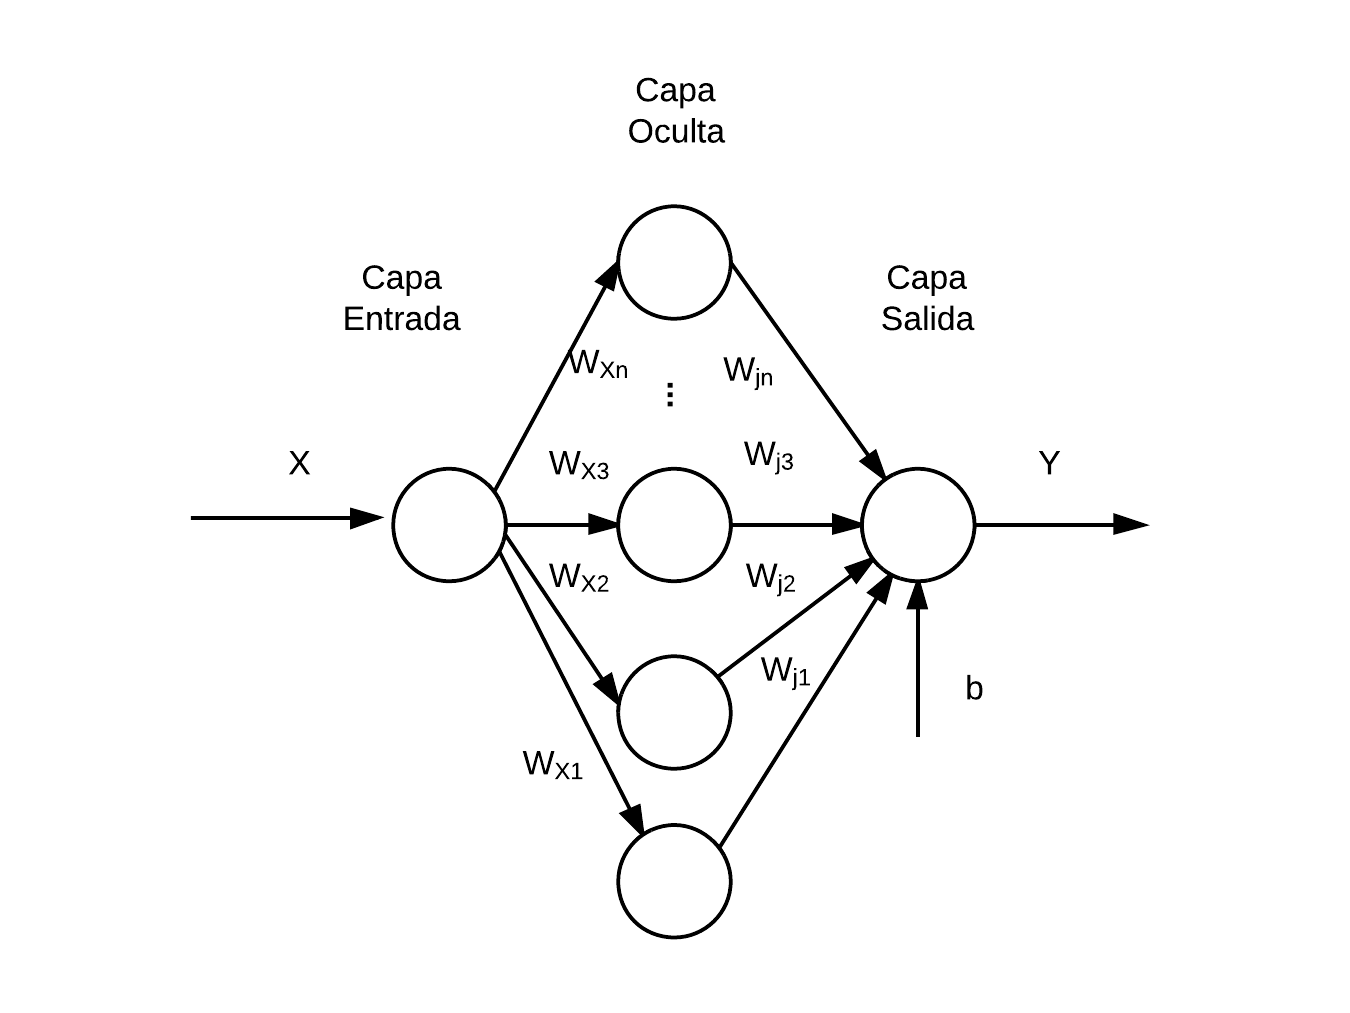
\includegraphics[width=\linewidth]{ann}
\\ {\footnotesize \textbf{Figura 1.} Arquitectura de red con una capa oculta.}
\end{center}

%En este trabajo se utilizó un filtro Butterworth de orden 5 discretizado por el %método de la transformada bilineal para eliminar las frecuencias no deseadas %provenientes de factores externos a la estructura.

}

%----------------------------------------------------------------------------------------
%	MATERIALS AND METHODS
%----------------------------------------------------------------------------------------

\headerbox{Descripción del experimento}{name=methods,column=0,below=introduction}{

\begin{footnotesize}

El método de análisis de vibración utilizado para este experimento fue el de desplazamiento de frecuencia, en el que la detección de los daños se realizar por medio de los cambios en las frecuencias naturales de la estructura. El método se basa en que la frecuencia de vibración es una función de la rigidez, de modo que un cambio en este parámetro causado por el deterioro de la estructura se refleja como una disminución en las frecuencias de vibración.\\

\textbf{Componentes de Sistema}
\begin{itemize}
	\item Acelerómetro ADXL335, 330 mV/g, $\pm$3,6 g.
	\item Intel Galileo, ADC AD7298 12 bits, 200 Hz.
	\item Filtro Digital.
	\item FFTW.
\end{itemize}

\end{footnotesize}


\begin{center}
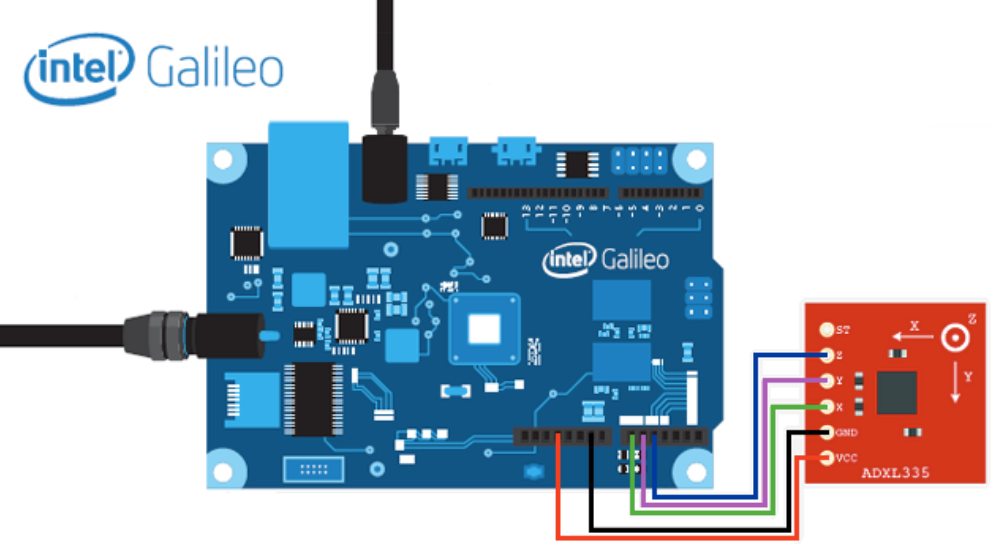
\includegraphics[width=0.6\linewidth]{galileo}

{\footnotesize \textbf{Figura 2.} Placa utilizada. Intel Galileo.}
\end{center}



}

%----------------------------------------------------------------------------------------
%	CONCLUSION
%----------------------------------------------------------------------------------------



%----------------------------------------------------------------------------------------
%	REFERENCES
%----------------------------------------------------------------------------------------

\headerbox{Referencias}{name=references,column=0,below=methods}{

\smaller % Reduce the font size in this block
%\renewcommand{\section}[2]{\vskip 0.05em} % Get rid of the default "References" section title
%\nocite{*} % Insert publications even if they are not cited in the poster

\begin{footnotesize}
{[1]} V. Reyes and M. Antonio, “Algoritmo backpropagation para redes neuronales: conceptos y aplicaciones,” Instituto Politécnico Nacional,España, 2007. \\
{[2]} F. J. Carrión Viramontes, A. Lozano Guzmán, M. Fabela Gallegos, D. Vázquez Vega, and J. A. Romero Navarrete, “Evaluación de Puentes Mediante el Análisis de Vibraciones”, Publicación Técnica, n.o 132, 1999.
\end{footnotesize}




%\bibliographystyle{unsrt}
%\bibliography{sample} % Use sample.bib as the bibliography file
}

%----------------------------------------------------------------------------------------
%	ACKNOWLEDGEMENTS
%----------------------------------------------------------------------------------------

%\headerbox{Acknowledgements}{name=acknowledgements,column=0,below=references, above=bottom}{

%\smaller % Reduce the font size in this block
%Fusce mattis tellus ac odio imperdiet lobortis. Cum sociis natoque penatibus et %magnis dis parturient montes, nascetur ridiculus mus. Phasellus commodo blandit %euismod. Ut porttitor cursus magna. Mauris adipiscing pellentesque ipsum nec %facilisis. Cras ornare bibendum bibendum. Ut a elit purus, vel adipiscing.
%} 

%----------------------------------------------------------------------------------------
%	RESULTS 1
%----------------------------------------------------------------------------------------

\headerbox{Transformada discreta de Fourier (DFT)}{name=results1,span=2,column=1,row=0}{ % To reduce this block to 1 column width, remove 'span=2'


\begin{footnotesize}
Para el caso en estudio, daños en estructuras, las mediciones de vibración en la estructura fueron procesados a través de la Transformada Discreta de Fourier, utilizando la biblioteca \textbf{\textit{FFTW}. }


\end{footnotesize}
\begin{center}
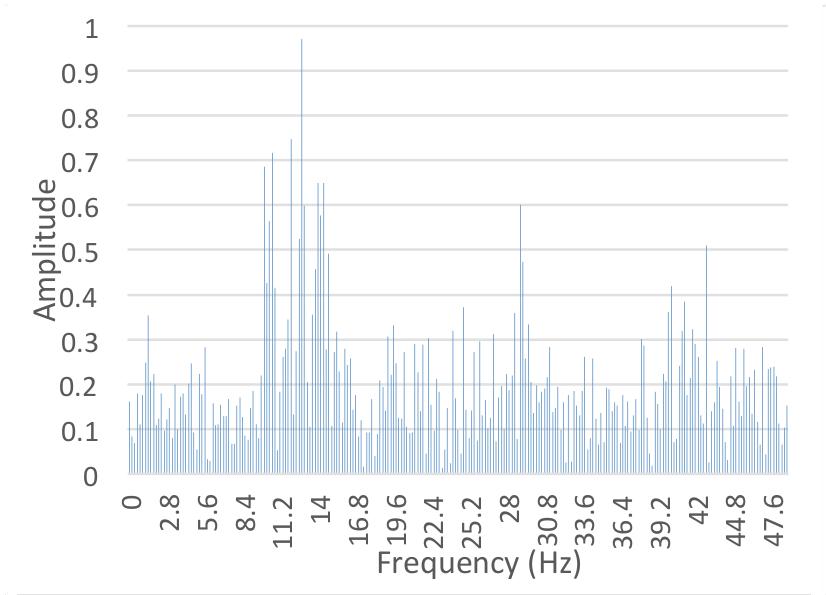
\includegraphics[width=0.5\linewidth]{fft}
\\ {\footnotesize \textbf{Figura 3.} DFT de datos de vibración, sin filtrar.}
\end{center}

%------------------------------------------------

%\begin{center}
%\begin{tabular}{l l l}
%\toprule
%\textbf{Treatments} & \textbf{Response 1} & \textbf{Response 2}\\
%\midrule
%Treatment 1 & 0.0003262 & 0.562 \\
%Treatment 2 & 0.0015681 & 0.910 \\
%Treatment 3 & 0.0009271 & 0.296 \\
%\bottomrule
%\end{tabular}
%\captionof{table}{Table caption}
%\end{center}
}

%----------------------------------------------------------------------------------------
%	RESULTS 2
%----------------------------------------------------------------------------------------

\headerbox{Resultados Entrenamiento}{name=results2,span=2,column=1,below=results1}{ % To reduce this block to 1 column width, remove 'span=2'



%------------------------------------------------




\begin{center}
\begin{tabular}{ccccc}
\toprule
Frecuencia (Hz) & Falta &Salida esperada &Salida Final & Predicción de Falta \\
\midrule
13,6 & 0 & 1 & 0,158297 & 0 \\
14,0 & 0 & 1 & 0,193457 & 0 \\
13,6 & 0 & 1 & 0,158297 & 0 \\
14,2 & 0 & 1 & 0,210621 & 0 \\
17,0 & 0 & 1 & 0,423674 & 0 \\
9,0 & 1 & -1 & -0,332459 & 1 \\
11,4 & 1 & -1 & -0,055948 & 1 \\
13,6 & 0 & 1 & 0,158297 & 0 \\
13,6 & 0 & 1 & 0,158297 & 0 \\
29,0 & 0 & 1 & 0,938729 & 0 \\
13,6 & 0 & 1 & 0,158297 & 0 \\
32,8 & 0 & 1 & 1,024909 & 0 \\
17,8 & 0 & 1 & 0,475995 & 0 \\
13,6 & 0 & 1 & 0,158297 & 0 \\
11,4 & 1 & -1 & -0,055948 & 1 \\
11,6 & 1 & -1 & -0,03496 & 1 \\
9,0 & 1 & -1 & -0,332459 & 1 \\
11,8 & 1 & -1 & -0,014281 & 1 \\
16,4 & 0 & 1 & 0,382073 & 0 \\
13,6 & 0 & 1 & 0,158297 & 0 \\
9,0 & 1 & -1 & -0,332459 & 1 \\
13,6 & 0 & 1 & 0,158297 & 0 \\
11,2 & 1 & -1 & -0,077247 & 1 \\
21,2 & 0 & 1 & 0,663058 & 0 \\
14,0 & 0 & 1 & 0,193457 & 0 \\
20,0 & 0 & 1 & 0,603023 & 0 \\
14,0 & 0 & 1 & 0,193457 & 0 \\
2,0 & 1 & -1 & -1,379501 & 1 \\
32,0 & 0 & 1 & 1,00856 & 0 \\
32,0 & 0 & 1 & 1,00856 & 0 \\
32,2 & 0 & 1 & 1,012728 & 0 \\
27,6 & 0 & 1 & 0,900674 & 0 \\
26,0 & 0 & 1 & 0,852009 & 0 \\
1,8 & 1 & -1 & -1,413221 & 1 \\
\bottomrule
\end{tabular}
\end{center}

%\begin{center}
%
\includegraphics[width=0.49\linewidth]{placeholder}
%
\includegraphics[width=0.49\linewidth]{placeholder}
%\captionof{figure}{Figure caption 1 (left); Figure caption 2 (right)}
%\end{center}

%------------------------------------------------
}
\headerbox{Conclusiones}{name=conclusion,column=1,row=0, span=2, below=results2,above=bottom}{

\

\begin{itemize}

\item El análisis en línea de faltas por medio de redes neuronales artificiales, bajo la técnica de DFT, permite su detección en tiempo real.
\item Los resultados muestran la viabilidad de un sistema empotrado para la detección de faltas utilizando redes neuronales artificiales.
\item La predicción de faltas por medio de la red fue satisfactoria para más de un 95 \% de los datos, lo que demuestre su validez como método de identificación de comportamiento anormal (falta).
\end{itemize}
}
%----------------------------------------------------------------------------------------

\end{poster}

\end{document}
